\section{The Potential of an Elliptic Ring}

\begin{figure}[h!]
    \begin{center}
        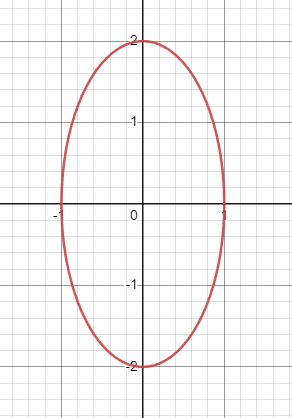
\includegraphics[scale=0.5]{resources/elliptic_ring.png}
        \caption{An elliptic ring.}
        \label{potential::elliptic_ring}
    \end{center}
\end{figure}

Consider an elliptic ring (see Figure~\ref{potential::elliptic_ring}) with
\begin{equation}
    \mu = \frac{M}{L}
\end{equation}
where \( \mu \) is the mass per unit length, \( M \) is the total mass of the ring and \( L \) is the perimeter of the ring.

The potential of a small segment of the ring is given by the equation
\begin{equation}
    \delta \Phi(\vec{r}) = -\frac{Gm_{\text{segment}}}{\left|\vec{r} - \vec{r}_{\text{segment}}\right|}
\end{equation}
The mass of the segment is
\begin{equation}
    m_{\text{segment}} = \mu \delta s
\end{equation}
where \( \delta s \) is the length of the small segment of the ellipse, so
\begin{equation}
    \delta \Phi(\vec{r}) = -\frac{G\mu \delta s}{\left|\vec{r} - \vec{r}_{\text{segment}}\right|}
\end{equation}
Therefore, the potential of the entire elliptic ring is simply
\begin{equation}
    \Phi_{\text{ring}}(\vec{r}) = G\mu \int \frac{\mathrm{d}s}{\left|\vec{r} - \vec{r}_{\text{segment}}\right|}
\end{equation}
In order to integrate, we will need to express the line element in coordinates that lie on the ellipse.
The Cartesian coordinates \( (x, y) \) of a point on the ellipse can be written as
\begin{align}
    x & = aR\cos{\theta} \\
    y & = bR\sin{\theta}
\end{align}
where \( a \) and \( b \) are the scale width and height of the ellipse respectively, \( R \) is the scale length and \( \theta \)
is a parameter that varies from \( 0 \) to \( 2\pi \). We want to get the differentials of these coordinates in terms of
\( d\theta \) to aid in the integration.
\begin{align}
    \mathrm{d}x & = -aR\sin{\theta} \mathrm{d}\theta \\
    \mathrm{d}y & = bR\cos{\theta} \mathrm{d}\theta
\end{align}
The line element \( \mathrm{d}s \) is hence given by
\begin{align}
    {\mathrm{d}s}^{2}    & = {\mathrm{d}x}^{2} + {\mathrm{d}y}^{2} \nonumber                                                      \\
                         & = a^2R^2\sin^2{\theta} {\mathrm{d}\theta}^2 + b^2R^2\cos^2{\theta} {\mathrm{d}\theta}^2 \nonumber      \\
                         & = R^2\left(a^2\sin^2{\theta} + b^2\cos^2{\theta}\right) {\mathrm{d}\theta}^2 \nonumber                 \\
                         & = R^2\left(a^2\left(1 - \cos^2{\theta}\right)+ b^2\cos^2{\theta}\right) {\mathrm{d}\theta}^2 \nonumber \\
                         & = R^2\left(a^2 - (a^2 - b^2)\cos^2{\theta}\right) {\mathrm{d}\theta}^2 \nonumber                       \\
                         & = a^2R^2\left(1 - \left(1 - \frac{b^2}{a^2}\right)\cos^2{\theta}\right) {\mathrm{d}\theta}^2 \nonumber \\
                         & = a^2R^2 \left(1 - e^2\cos^2{\theta}\right) {\mathrm{d}\theta}^2 \nonumber                             \\
    \implies \mathrm{d}s & = aR\sqrt{1 - e^2\cos^2{\theta}} \mathrm{d}\theta
\end{align}
where \( e \) is the eccentricity of the ellipse equal to \( e = \sqrt{1 - \frac{b^2}{a^2}} \).
Finally, the potential \( \Phi_{\text{ring}}(\vec{r}) \) evaluated at \( \vec{r} \) is given by the integral
\begin{equation}
    \Phi_{\text{ring}}(\vec{r}) = -G \mu a R \int_{0}^{2\pi} \frac{\sqrt{1 - e^2\cos^2{\theta}}}{\left|\vec{r} - \vec{r}_{\text{ellipse}}\right|} \,\,{} \mathrm{d}\theta
\end{equation}
The potential in terms of Cartesian coordinates \( (x, y) \) can be written as
\begin{equation}
    \Phi_{\text{ring}}(x, y) = -G \mu R \int_{0}^{2\pi} \frac{\sqrt{1 - e^2\cos^2{\theta}}}{\sqrt{{(x - x_{\text{ellipse}})}^{2} + {(y - y_{\text{ellipse}})}^{2}}} \,\,{} \mathrm{d}\theta
\end{equation}
Substituting in for \( x \) and \( y \) their parametric forms we obtain
\begin{equation}
    \Phi_{\text{ring}}(x, y) = -G \mu a R \int_{0}^{2\pi} \frac{\sqrt{1 - e^2\cos^2{\theta}}}{\sqrt{{(x - aR\cos{\theta})}^{2} + {(y - bR\sin{\theta})}^{2}}} \,\,{} \mathrm{d}\theta
\end{equation}
This only applies for ellipses coaxial with the Cartesian coordinate axes, so in order to get the potential of a rotated ellipse,
we want the coordinates of the ellipse rotated by an angle \( \alpha \), say anti-clockwise
\begin{align}
    \begin{pmatrix}
        x' \\ y'
    \end{pmatrix} & = \begin{pmatrix}
                          \cos{\alpha} & -\sin{\alpha} \\
                          \sin{\alpha} & \cos{\alpha}
                      \end{pmatrix} \begin{pmatrix}
                                        x \\ y
                                    \end{pmatrix}                              \\
                    & = \begin{pmatrix}
                            \cos{\alpha} & -\sin{\alpha} \\
                            \sin{\alpha} & \cos{\alpha}
                        \end{pmatrix} \begin{pmatrix}
                                          aR\cos{\theta} \\ bR\sin{\theta}
                                      \end{pmatrix} \nonumber             \\
    \begin{pmatrix}
        x' \\ y'
    \end{pmatrix} & = R\begin{pmatrix}
                           a\cos{\alpha}\cos{\theta} - b\sin{\alpha}\sin{\theta} \\
                           a\sin{\alpha}\cos{\theta} + b\cos{\alpha}\sin{\theta}
                       \end{pmatrix} \label{potential::rotated_ellipse_cartesian}
\end{align}
% TODO: I don't know if this is correct. theta is the angle of the ellipse, not the angle of rotation, so the line element might
% not be the same.
So the potential of a rotated elliptic ring is
\begin{equation}
    \Phi_{\text{ring}}(x, y) = -G \mu a R \int_{0}^{2\pi} \frac{\sqrt{1 - e^2\cos^2{\theta}}}{\sqrt{{(x - x')}^{2} + {(y - y')}^{2}}} \,\,{} \mathrm{d}\theta
\end{equation}
where \( (x', y') \) are given by Equation~\ref{potential::rotated_ellipse_cartesian}.